\chapter{Visitor}
\section{Intento}

Rappresentare un'operazione da eseguire sugli elementi di una struttura di oggetti. Il Visitor permette di definire una nuova operazione senza modificare le classi degli elementi su cui opera.


%---
\section{Struttura}

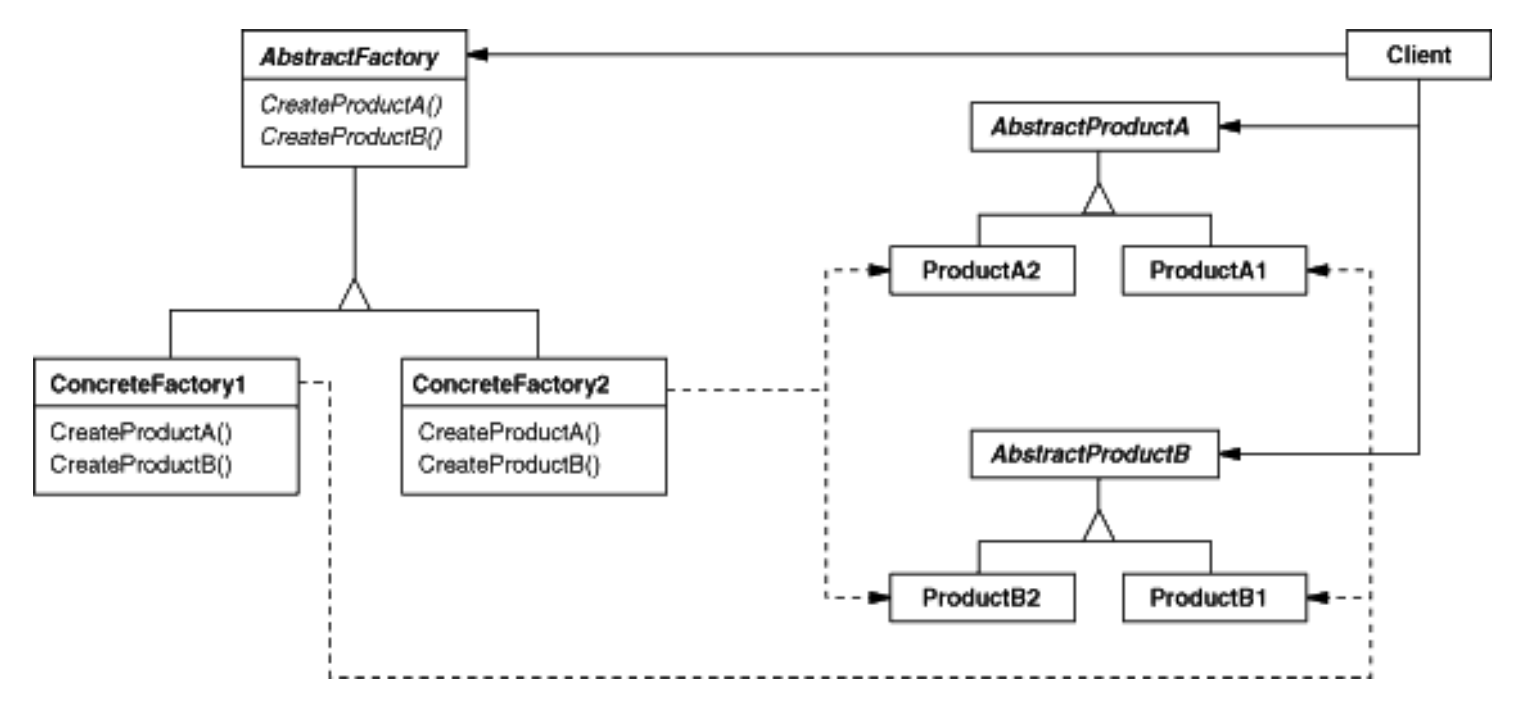
\includegraphics[width=\textwidth]{/Users/matt/Documents/GitHub/Design-Pattern-ITA/Visitor/Structure1}


%---
\section{Timeline}

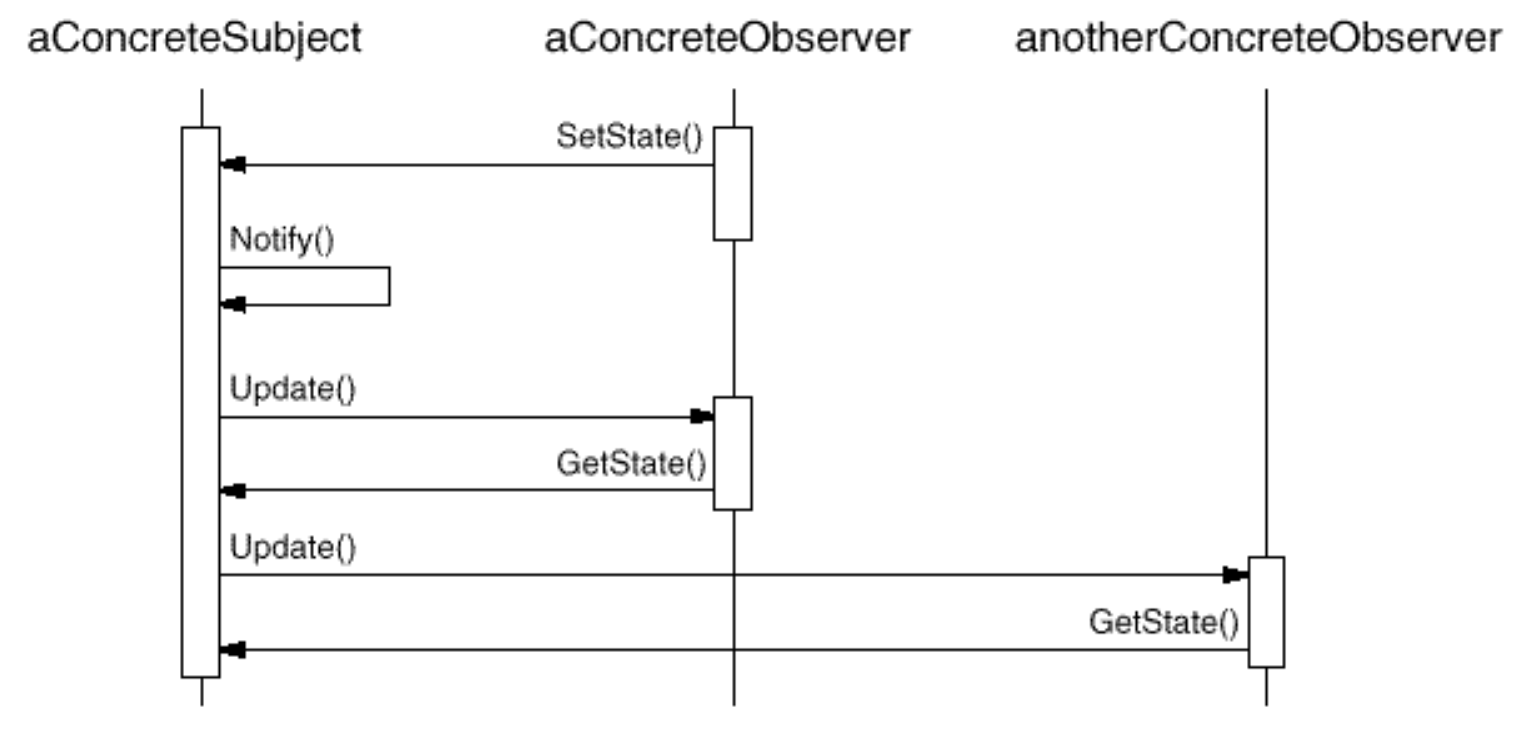
\includegraphics[width=\textwidth]{/Users/matt/Documents/GitHub/Design-Pattern-ITA/Visitor/Timeline1}


%---
\section{Implementazione}

\subsection{Doppio invio.} 
Il pattern Visitor consente di aggiungere operazioni alle classi senza modificarle. Il visitatore ottiene ciò utilizzando una tecnica chiamata double-dispatch.

Nei linguaggi a single-dispatch, due criteri determinano quale operazione soddisferà una richiesta:

\begin{itemize}
    \item nome della richiesta
    \item tipo di destinatario
\end{itemize}

"Doppio invio" significa semplicemente che l'operazione che viene eseguita dipende dal tipo di richiesta e dai tipi di due destinatari.

Accept è un'operazione a doppio invio. Il suo significato dipende da due tipi:

\begin{itemize}
    \item quello del Visitator
    \item quello di Element
\end{itemize}

\subsection{Chi è responsabile dell'attraversamento della struttura dell'oggetto?}
Spesso la struttura dell'oggetto è responsabile dell'iterazione.

Una raccolta itererà semplicemente sui suoi elementi, chiamando l'operazione Accept uno per ciascuno. Un composto normalmente attraverserà se stesso facendo in modo che ogni operazione Accept attraversi i figli dell'elemento e chiami Accept su ciascuno di essi in modo ricorsivo.

Un'altra soluzione consiste nell'utilizzare un iteratore per visitare gli elementi.


%---
\section{Esempio Java}
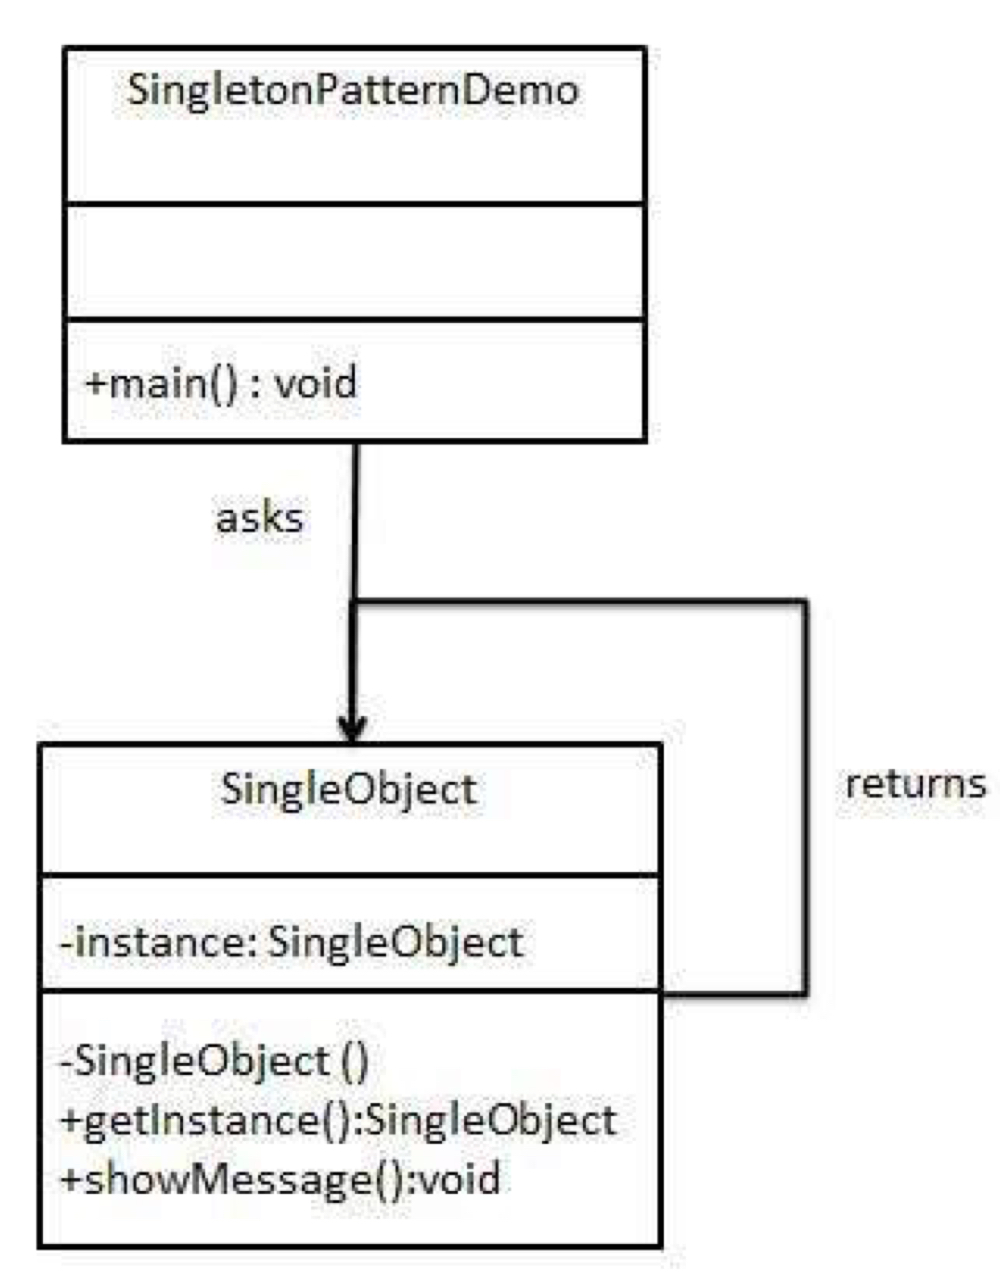
\includegraphics[width=\textwidth]{/Users/matt/Documents/GitHub/Design-Pattern-ITA/Visitor/Example1}

\subsection{ComputerPart.java}
\begin{lstlisting}[language=java]
    public interface ComputerPart {
        void accept(ComputerPartVisitor cpv);
    }
\end{lstlisting}

\subsection{ComputerPartVisitor.java}
\begin{lstlisting}[language=java]
    public interface ComputerPartVisitor {
        void visit(Computer computer);
        void visit(Monitor monitor);
        void visit(Mouse mouse);
        void visit(Keyboard keyboard);
    }
\end{lstlisting}

\subsection{Computer.java}
\begin{lstlisting}[language=java]
    public class Computer implements ComputerPart {
        ComputerPart[] parts;
    
        public Computer() {
            parts = new ComputerPart[] {new Keyboard(),
                                        new Mouse(),
                                        new Monitor()};
        }
    
        @Override
        public void accept(ComputerPartVisitor cpv) {
            for (int i = 0; i < parts.length; i++) {
                parts[i].accept(cpv);
            }
            cpv.visit(this);
        }
        
    }
\end{lstlisting}

\subsection{Keyboard.java}
\begin{lstlisting}[language=java]
    public class Keyboard implements ComputerPart{

        @Override
        public void accept(ComputerPartVisitor cpv) {
            cpv.visit(this);
        }
        
    }
\end{lstlisting}

\subsection{Monitor.java}
\begin{lstlisting}[language=java]
    public class Monitor implements ComputerPart{

        @Override
        public void accept(ComputerPartVisitor cpv) {
            cpv.visit(this);
        }
        
    }
\end{lstlisting}

\subsection{Mouse.java}
\begin{lstlisting}[language=java]
    public class Mouse implements ComputerPart{

        @Override
        public void accept(ComputerPartVisitor cpv) {
            cpv.visit(this);
        }
        
    }
\end{lstlisting}

\subsection{ComputerPartDisplayVisitor.java}
\begin{lstlisting}[language=java]
    public class ComputerPartDisplayVisitor implements ComputerPartVisitor {

        @Override
        public void visit(Computer computer) {
            System.out.println("Visito computer");
        }
    
        @Override
        public void visit(Monitor monitor) {
            System.out.println("Visito monitor");
            
        }
    
        @Override
        public void visit(Mouse mouse) {
            System.out.println("Visito mouse");
            
        }
    
        @Override
        public void visit(Keyboard keyboard) {
            System.out.println("Visito keyboard");
            
        }
        
    }
    
\end{lstlisting}

\subsection{main}
\begin{lstlisting}[language=java]
    public static void main(String[] args) {
        ComputerPart computer = new Computer();
        computer.accept(new ComputerPartDisplayVisitor());
    }
\end{lstlisting}